\documentclass{standalone}

\usepackage[latin1]{inputenc}
\usepackage{tikz}
\usetikzlibrary{arrows,automata}
\begin{document}
\pagestyle{empty}


% Set the overall layout of the tree
\tikzstyle{level 1}=[level distance=11em, sibling distance=10ex]

% Define styles for bags and leafs
\tikzstyle{bag} = [rectangle, draw, text width=10em, text centered, thick]

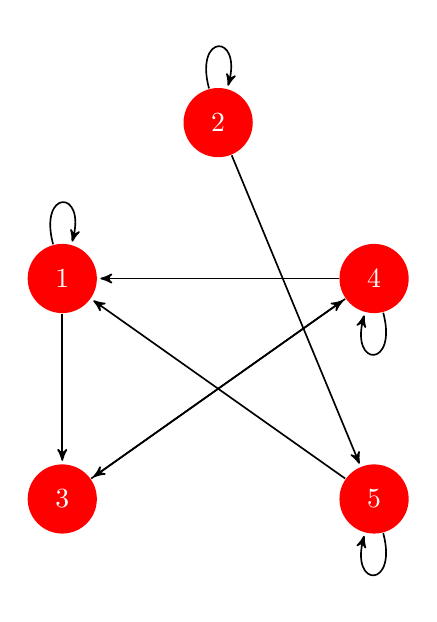
\begin{tikzpicture}[->,>=stealth',shorten >=1pt,auto,node distance=2.8cm,
                    semithick]
  \tikzstyle{every state}=[fill=red,draw=none,text=white]

  \node[state] (A)                    {$1$};
  \node[state] (B) [above right of=A] {$2$};
  \node[state] (C) [below of=A] {$3$};
  \node[state] (D) [below right of=B] {$4$};
  \node[state] (E) [below of=D]       {$5$};

  \path (A) edge [loop above] node {} (A)
            edge              node {} (C)
        (B) edge [loop above] node {} (B)
            edge              node {} (E)
        (C) edge              node {} (D)
        (D) edge [loop below] node {} (D)
            edge              node {} (A)
            edge              node {} (C)
        (E) edge [loop below] node {} (E)
            edge              node {} (A);
\end{tikzpicture}

\end{document}
